% Klassifiziert den Dokumenten-Typ
% Doku: http://exp1.fkp.physik.tu-darmstadt.de/tuddesign/
% Farben: http://www.tu-darmstadt.de/media/medien_stabsstelle_km/services/medien_cd/das_bild_der_tu_darmstadt.pdf
%  bigchapter: Chapter haben doppelte Schriftgröße
%  linedtoc: Linien im Inhaltsverzeichnis wie bei Überschriften
%  colorbacktitle: Der Dokumenten-Titel wird mir der Accentfarbe hinterlegt
\documentclass[bigchapter,colorback,accentcolor=tud4b,linedtoc,11pt]{tudreport}

% Input Dokument hat das Encoding UTF-8
\usepackage[utf8]{inputenc}
% Wichtiges Paket für Links und verlinktes Inhaltsverzeichnis
\usepackage[ngerman]{hyperref}
% Paket für Fußnoten
\usepackage[stable]{footmisc}
% Paket für amsmath (aligned mathe formeln)
\usepackage{amsmath}
% Paket für Bibliotheks-Verzeichnis, square: Verwende eckige statt runde klammern
% \usepackage[square]{natbib}
% Paket zum Plotten von Datensätzen
\usepackage{pgfplots}
\pgfkeys{%
  /pgfplots/Streudaten/.style={%
    /pgf/number format/use comma,
    legend pos=north east,
    xlabel=Streuvektor s in 1/nm,
    x tick label style={/pgf/number format/1000 sep=},
    ylabel=$I\cdot s^{2}$,
    y tick label style={/pgf/number format/1000 sep=},
    width=0.38\linewidth,
    height=0.40\linewidth,
    scale only axis,
    xmin=0,
    xmax=0.44,
    grid=both,
    ymin=-10,
    %ymax=0.0045,
    tick align=outside,
    tickpos=left,
    minor x tick num=3,
    minor y tick num=4,
    minor grid style={dotted,thin}
  }
}

\pgfkeys{%
  /pgfplots/Autokorrel/.style={%
    /pgf/number format/use comma,
    legend pos=north east,
    xlabel=u  in  nm,
    x tick label style={/pgf/number format/1000 sep=},
    ylabel=$K(u)$ in $\frac{e}{nm^{6}}$,
    y tick label style={/pgf/number format/1000 sep=},
    width=0.38\linewidth,
    height=0.30\linewidth,
    scale only axis,
    xmin=0,
    xmax=25,
    grid=both,
    ymin=-105,
    ymax=155,
    tick align=outside,
    tickpos=left,
    minor x tick num=3,
    minor y tick num=4,
    minor grid style={dotted,thin}
  }
}

\pgfkeys{%
  /pgfplots/tabh/.style={%
    /pgf/number format/use comma,
    legend pos=north east,
    x tick label style={/pgf/number format/1000 sep=},
    xlabel=Unterkühlung in $K$,
    y tick label style={/pgf/number format/1000 sep=},
    width=0.38\linewidth,
    height=0.30\linewidth,
    scale only axis,
    xmin=0,
    xmax=100,
    grid=both,
    ymin=3,
    ymax=6,
    tick align=outside,
    tickpos=left,
    minor x tick num=3,
    minor y tick num=4,
    minor grid style={dotted,thin}
  }
}

% Anhänge für Original-Messdaten
\usepackage{fancyvrb}

% redefine \VerbatimInput
\RecustomVerbatimCommand{\VerbatimInput}{VerbatimInput}%
{fontsize=\footnotesize,
 %
 frame=lines,  % top and bottom rule only
 framesep=2em, % separation between frame and text
 fontsize=\scriptsize,
 %
 labelposition=topline,
 %
 commandchars=\|\(\), % escape character and argument delimiters for
                      % commands within the verbatim
 commentchar=*        % comment character
}

% Polar Plots
\usetikzlibrary{pgfplots.polar}
% Verwende deutsche Bezeichner für Inhaltsverzeichnis, ... (ngerman = New German: neue Rechtschreibung)
\usepackage{ngerman}
% Deutsche Zahlen (entfernt z.B. das Leerzeichen nach einem Dezimal-Komma)
\usepackage{ziffer} 

\usepackage[verbose]{placeins}

%wegen Grafikverschiebung hinzugefügt
\usepackage{float}

%\usepackage{graphicx}
%\usepackage{caption}
\usepackage{subcaption} %Für subfigures

% PDF-Optionen
\hypersetup{%
  pdftitle={TU Darmstadt \- Physikalisches Praktikum für Fortgeschrittene},
  pdfauthor={Esra Bauer und Sören Link},
  pdfsubject={Versuch 3.21},
  pdfview=FitH,
}
% Nummeriere formeln in Subsections einzeln
% Kleines makro zur assymetrischen Fehlerangabe

% Entspricht-Zeichen
\usepackage{scalerel}

\newcommand\equalhat{%
\let\savearraystretch\arraystretch
\renewcommand\arraystretch{0.3}
\begin{array}{c}
\stretchto{
    \scalerel*[\widthof{=}]{\wedge}
    {\rule{1ex}{3ex}}%
}{0.5ex}\\ 
=%
\end{array}
\let\arraystretch\savearraystretch
}
%BEGINN TITELSEITE

\title{Röntgenkleinwinkelstreuung an teilkristallinen Polymeren}

\subtitle{Esra Bauer  \\Sören Link}

\subsubtitle{Betreuer: Jan Gabriel \hfill Versuchsdatum: 24. November 2014}

\author{Esra Bauer, Sören Link}

%\settitlepicture{img/title.jpg}

\institution{Physikalisches Praktikum \\für Fortgeschrittene \\ Versuch 3.21}

\date{\today}


%ENDE TITELSEITE

\begin{document}
%ANFANG DOKUMENT

%Titelseite einfügen
\maketitle

%Inhaltsverzeichnis einfügen
\tableofcontents

%ANFANG INHALT

\chapter{Einleitung}

In diesem Versuch wird die Struktur von PET, einem Polymer, welcher uns in Form von Getränkeflaschen bekannt ist, näher untersucht. Das Interessante dabei ist, dass es sich weder um einen rein amorhpen Stoff, wie z.B. Fensterglas, noch um einen klassischen kristallinen Stoff handelt. Er besitzt vielmehr die Fähigkeit, sich teilweise kristallin zu ordnen, wobei dies stark von der Historie des Temperaturverlaufs abhängt. Daher werden im Versuch Proben des Materials untersucht, die unterschiedlich getempert wurden. Mithilfe der Röntgenkleinwinkelstreuung sollen Rückschlüsse auf die Struktur der Proben ermöglicht werden.

\chapter{Grundlagen}
\section{Polymere}

Allgemein handelt es sich bei Polymeren um Makromoleküle, die aus Kettenmolekülen oder verzweigten Molekülen aufgebaut sind. Diese Makromoleküle können aus bis zu mehreren hunderttausend Bausteinen bestehen, die man Monomere nennt. Die Länge der Polymere bestimmt dabei den Polymerisationsgrad und man unterscheidet Thermoplasten, Duroplasten und Elastomere, wobei bei ersteren die Makromoleküle kettenförmig sind, bei den Duroplasten stärker und bei Elastomeren schwächer vernetzt. Die physikalischen Eigenschaften sind dementsprechend unterschiedlich: Elastomere sind elastisch dehnbar und Duroplasten auch bei höheren Temperaturen starr bzw.\ im Vergleich eher spröde. 

Interessant sind für diesen Vesuch vor allem die Gruppe der Thermoplasten, zu denen auch das zu untersuchende PET gehört. Sie lassen sich, wie der Name sagt, einschmelzen und umformen. In der Schmelze liegen die Kettenmoleküle ungeordnet vor. Man spricht von einem Gaußschen Knäuel; der sog. Gyrationsradius ist proportional zur Wurzel des Molekulargewichts. Das Quadrat des Gyrationsradius ist definiert als der mittlere quadratische Abstand der Monomere zum Schwerpunkt des Polymers. Abhängig von der Abkühlgeschwindigkeit und -temperatur treten dann zwei wesentliche Übergänge auf: Der Glasübergang und (teilweise) Kristallisation.

\section{Glasübergang}

Kühlt man geschmolzene Thermoplasten schnell wieder ab, reicht die Zeit für die Kettenmoleküle, aus denen sie aufgebaut sind, nicht aus um sich regelmäßig anzuordnen, d.h.\ die Knäuelstruktur erstarrt und bleibt unregelmäßig. Es entsteht ein amorpher Festkörper, wie z.B. Fensterglas. Es handelt sich dabei nicht um einen thermodynamischen Phasenübergang, da keine fest definierte Temperatur für den Glasübergang existiert, sondern in der Realität ein allmählicher Übergang stattfindet, der zudem von der Abkühlgeschwindigkeit abhängt. Trägt man die einem Festkörper zugeführte Wärme $Q_{zu}$ über seiner Temperatur auf, wird dies als Aufweichung sichtbar:


\begin{figure}[h] 
  \centering
     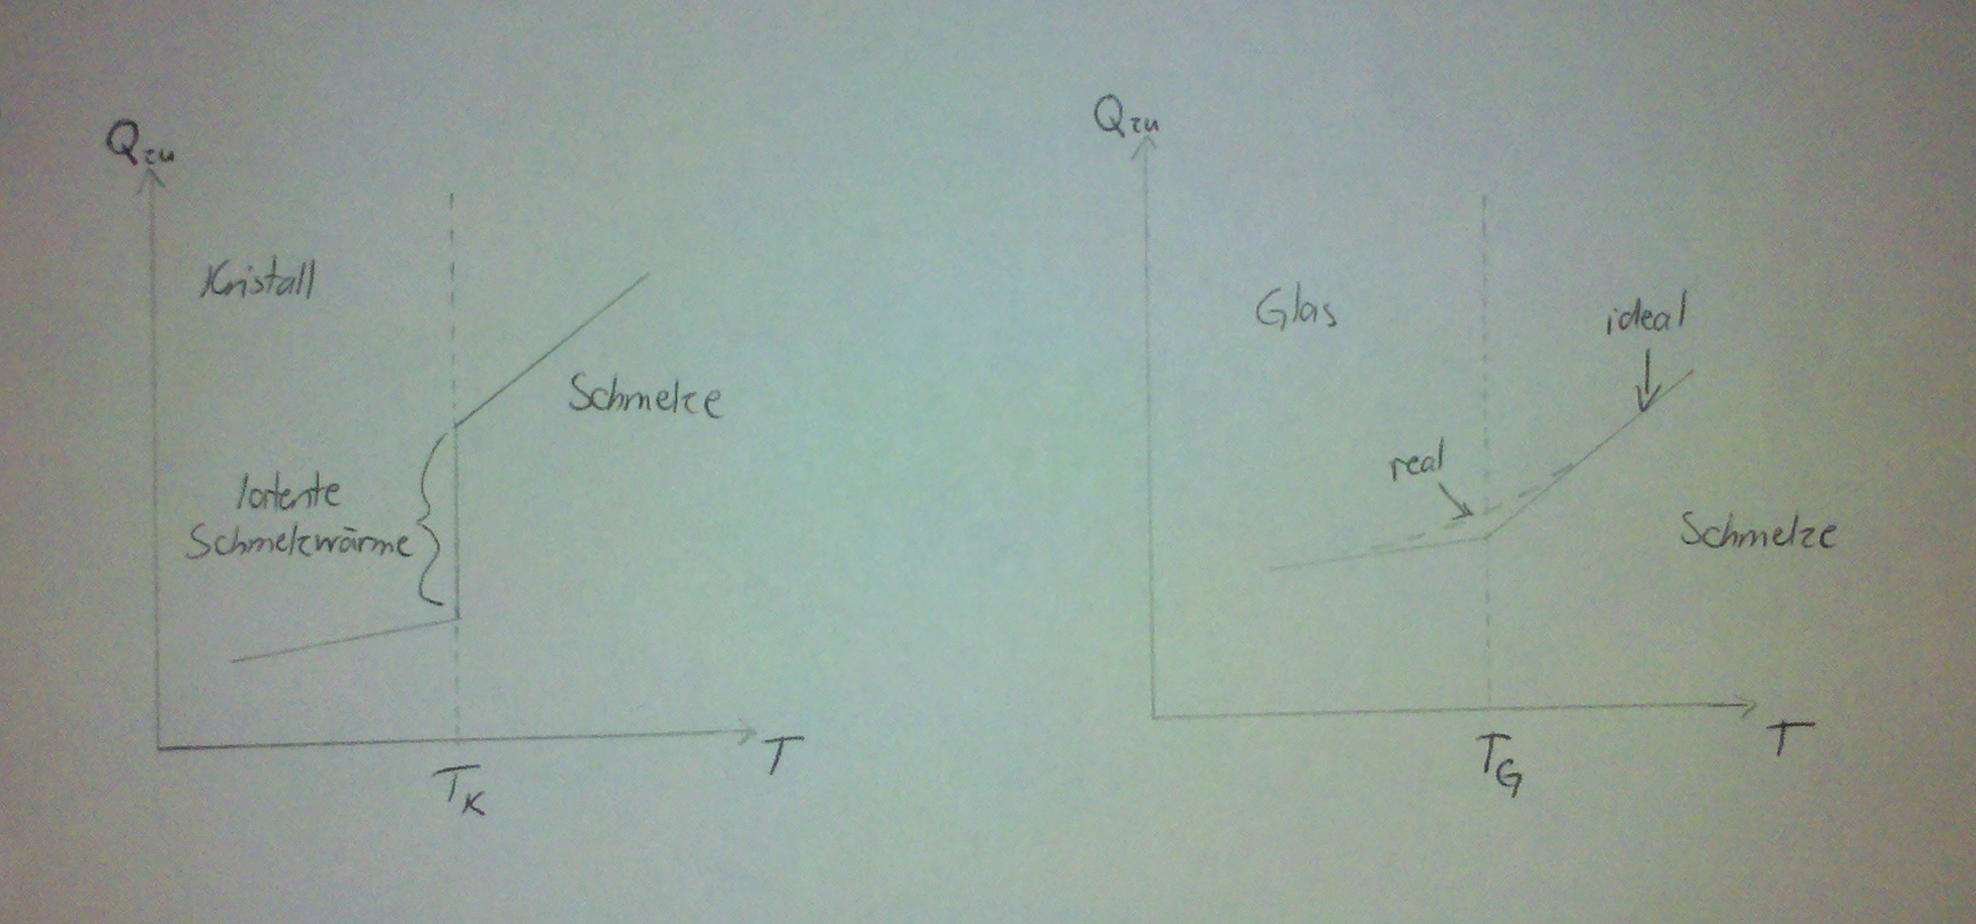
\includegraphics[width=0.7\textwidth]{data/glastemperatur.jpg}
  \caption{Zugeführte Wärme $Q_{zu}$ über der Temperatur des Festkörpers. Links ist der Schmelzprozess eines kristallinen Festkörpers zu sehen, rechts der eines amorphen Festkörpers.}
  \label{fig:Bild1}
\end{figure}

Im $Q_{zu}$-T-Diagramm kann der Glasübergang für eine ideale geringe Aufweichung der Glasübergangstemperatur allerdings wie ein Phasenübergang zweiter Ordnung erscheinen. Dennoch ist hier deutlich der Unterschied zum Kristallübergang, der ein Phasenübergang erster Ordnung ist, zu sehen. Charakteristisch für den Kristallübergang ist die latente Schmelzwärme, die sich nicht in einer Temperaturerhöhung zeigt, sondern für die Auflösung der kristallinen Strukturen benötigt wird. Am Diagramm für den Glasübergang wird auch deutlich, dass sich hieraus die Glasübergangstemperatur nur schwer bestimmen lässt. Eine alternative Methode hierfür ist deswegen die Zuordnung einer bestimmten Viskosität zur Glasübergangstemperatur.

\section{Kristallinität in Polymeren}

Wenn man die Abkühlgeschwindigkeit senkt bzw.\ den geschmolzenen Thermoplasten einige Zeit bei konstanter Temperatur hält und die Voraussetzung gegeben ist, dass die Kristallisationstemperatur höher als die Glasübergangstemperatur liegt, können die Kettenmoleküle sich gebietsweise regelmäßig strukturieren. Man spricht dann von Kristallisation. Energetisch am günstigen wäre ein Zustand, in dem sämtliche Ketten vollständig entfaltet parallel aneinanderliegen würden. Dies lässt sich dadurch erklären, dass zwischen den Ketten Van-der-Waals-Kräfte wirken, die vor allem bei kleinem Teilchenabstand zum Tragen kommen und bei größerem Abstand vernachlässigbar schwach werden. Folglich erfährt eine Kette, die nicht parallel zur nächsten liegt, in der Regel Kräfte verschiedener anderer Ketten in verschiedene Richtungen, d.h.\ der Zustand ist nicht stabil. Liegen die Ketten allerdings parallel, wird die Van-der-Waals-Kraft pro Kette auf ihren Nachbarn maximal, da jedes Teilchen den kleinstmöglichen Abstand zum entsprechenden Teilchen der Nachbarkette hat.

Zunächst erfolgt eine Keimbildung, d.h.\ es bilden sich sog. Kristallite (lokale Ordnungszustände mit einer typischen Größe von 15-100 nm), in denen die Molekülketten großteils parallel liegen. Großteils deshalb, weil sich die langen Molekülketten, obwohl dies energetisch am günstigsten wäre, nicht vollständig entfalten können. In der Realität falten sich die Ketten und liegen an den Enden und Schlaufen oft ungeordnet vor. Diese Kristallite können nun weiter wachsen, wobei zu beachten ist, dass sie dies bevorzugt in eine ausgezeichnete Richtung tun, da zum einen an den Seiten, an denen die Schlaufen liegen, kein Wachstum stattfinden kann, da hier amporhe Bereiche außenliegend sind, und zum andern die Richtung des größten Temperaturgradienten bevorzugt wird. Somit wächst der Kristallit in die Länge, es entstehen sog. Lamellen, also längliche Kristallstrukturen, in denen die Molekülketten quer zur Längsachse der Lamellen angeordnet sind.

Beim weiteren Wachstum muss unterschieden werden, unter welchem Temperaturbedingungen die Kristallisation erfolgt. Besteht ein starkes Temperaturgefälle, ordnen sich die Lamellen parallel an. Dies ist aber im Rahmen des Versuchs nicht weiter von Belang, da die Proben unter weitgehend isotropen Temperaturbedingen kristallisiert wurden, wobei sich die Lamellen radialsymmetrisch anordnen. Man spricht bei diesen radialsymmetrischen Strukturen von Sphärolithen. Eine vollständige Kristallisation ist in Polymeren nicht möglich, da bereits die Grundbausteine, die Kristallite, amorphe Randbereiche besitzen, an denen sich keine geordnete Struktur anlagern kann. Die Kristallisation lässt sich aber durch Additive signifikant steigern, auch Verunreinigungen und nicht ganz aufgeschmolzene kristalline Bestandteile können die Kristallisation verbessern.

Die Wachstumsrate der Kristallite ist durch $u \propto \cdot e^{-\frac{B_0}{T^{\infty}_{f}-T}-\frac{T_A}{T-T_V}}$ mit $B_0:$ Materialkonstante, $T^{\infty}_{f}-T:$ Gleichgewichtsschmelztemperatur, $T_V:$ Vogel-Temperatur, $T_A:$ Aktivierungstemperatur und $T:$ Temperatur der Probe beim Kristallisieren gegeben.

\section{Röntgenstreuung}

Unter Röntgenstrahlung versteht man elektromagnetische Strahlung hoher Energie (zwischen 100 eV und einigen MeV), deren Wellenlängen entsprechend zwischen 10$^{-12}$ und 10$^{-8}$ liegen. Sie lässt sich beispielsweise mit einem Synchrotron oder einer Röntgenröhre erzeugen, wobei im Folgenden letztere verwendet wird und daher hier kurz auf die Funktionsweise eingegangen werden soll. Im Wesentlichen besteht die Röntgenröhre aus einer beheizten Kathode, die freie Elektronen erzeugt, sowie aus einer Anode, die gegenüber der Kathode eine Hochspannung von 40kV besitzt. Die Elektronen werden also zur Anode beschleunigt, was in zwei Arten von Strahlung resultiert, da zum einen Wechselwirkung der Elektronen mit dem elektromagnetischen Feld der Anode stattfindet, wobei die Elektronen abgelenkt bzw.\ gebremst werden (dies verursacht ein kontinuierliches Spektrum der sog. Bremsstrahlung), und zum andern die energiereicheren Elektronen Hüllenelektronen aus dem Anodematerial herausschlagen können. Der Effekt ist, dass ein Hüllenelektron der nächsten Schale nachrückt und genau die Energiedifferenz der beiden Schalen in Form von elektromagnetischer Strahlung frei wird. Es entsteht zusätzlich ein diskretes Spektrum der charakteristischen Röntgenstrahlung. Ein Übergang der L-Schale zur K-Schale wird dabei als $K_{\alpha}$-Linie bezeichnet, ein Übergang der M-Schale zur K-Schale als $K_{\beta}$-Linie usw. Die Lage der Linien sind dabei vom Anodenmaterial abhängig, welches in diesem Fall Kupfer ist. 

Alle Messungen werden mit einer sog. Kratky-Kompakt-Kamera durchgeführt. Sie besteht aus einem evakuierbaren Gehäuse (Betriebsdruck ca. 38 mbar), welches einseitig auf der Röntgenröhre aufliegt und an der anderen Seite einen per Schrittmotor fein verschiebbaren Szintillationsdetektor vorgeschaltet hat. An beiden Enden ist das Gehäuse mit 0,25 mm dicken Berylliumfenstern verschlossen, die der Röntgenstrahl durchdringt. Vor der Strahlungsquelle befindet sich zunächst das Kollimationssystem, ein sog. Blockkollimationssystem, welches aus drei rechteckigen, genau geschliffenen Blöcken besteht, wobei zwei Blöcke den Strahl nach oben begrenzen und einer nach unten. Der Strahl passiert zuerst den Eingangspalt (dies ist der vertikale Abstand der in Strahlrichtung ersten beiden Blöcke, welcher auf etwa 80 µm eingestellt wird) und danach den letzten oberen Block, welcher gemeinsam mit dem mittleren Block die Strahlebenen bestimmt und Streustrahlung unterdrückt. So kollimiert, trifft der Strahl auf die Probe (bzw.\ passiert bei der ersten Messung den leeren Probenhalter) und wird dann auf das Austrittsfenster gestreut. Bei den Messungen mit Probe wird der Primärstrahl, d.h.\ der nicht gestreute Strahl, durch einen metallenen Beamstop blockiert, um ein direktes Auftreffen auf den Detektor zu verhindern, da dieser dadurch zerstört werden würde. Der Abstand der Probe zum Detektor beträgt 20 cm.

\section{Streuung an zweiphasigen Schichtsystemen}
In einem idealen zweiphasigen Schichtsystem wechseln sich amorphe und kristalline Bereiche periodisch ab, wobei die Dichten in den jeweiligen Schichten als konstant und die Übergänge zwischen beiden Schichten als infinitesimal klein angenommen werden.

\begin{figure}[h] 
  \centering
     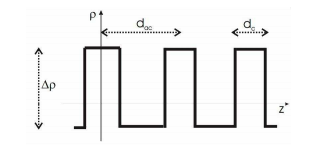
\includegraphics[width=0.4\textwidth]{img/uebergaenge.png}
     \caption{Schematische Darstellung der Elektronendichte-Verteilung in einem idealen zweiphasigen Schichtsystem \cite{anleitung}.}
\end{figure}

Die Elektronendichte der kristallinen und Amorphen Bereiche ergibt sich direkt aus der Furiertransformation der Amplitude der gestreuten Röntgenstrahlung. Leider können wir die Amplitude nicht direkt messen, wir messen lediglich die Intensität der gestreuten Strahlung $I(q) = A(\vec{q}) \cdot A^{*}(\vec{q})$.

Durch Einsetzen von $A(\vec{q}) = b_e \cdot \frac{A_0}{R} \int_{V} \rho(\vec{r}) \cdot e^{i\vec{q}\vec{r}}d\vec{r}$ \cite{anleitung} ergibt sich:

\begin{align*}
  I(q) &= b_{e}^{2} \cdot \frac{A_{0}^{2}}{R^2} \left( \int \rho(\vec{r}) \cdot e^{i\vec{q}\vec{r}}d\vec{r}\right) \left(\int \rho(\vec{r}^{\,\prime}) \cdot e^{-i\vec{q}\vec{r}^{\,\prime}}d\vec{r}^{\,\prime}\right),\\
  \text{Substition} \ \vec{u} &= \vec{r}^{\,\prime} - \vec{r},\\
  I(q) &= b_{e}^{2} \cdot \frac{I_{0}}{R^2} \int\left(\int \rho(\vec{r})\rho(\vec{u} + \vec{r}) d\vec{r}\right) \ e^{-i\vec{q}\vec{u}}d\vec{u},\\
  I(q) &= b_{e}^{2} \cdot \frac{I_{0}}{R^2} \int \Gamma_{\rho}(\vec{r})\ e^{-i\vec{q}\vec{u}} d\vec{u},\\
  \text{mit}\  \Gamma_{\rho}(\vec{r}) :&= \int \rho(\vec{r})\rho(\vec{u} + \vec{r}) d\vec{r}
\end{align*}
$\Gamma_{\rho}(\vec{r})$ ist dabei die Autokorrelationsfunktion der Elektronendichte (Patterson-Funktion).

Die Elektronenverteilung kann also durch Furiertransformation aus der Autokrellationsfunktion gewonnen werden.

In einem idealen zweiphasigen system würde die Autokorrelatonsfunktion einer Sägezahnfunktion entsprechen, allerdings setzen in diesem Versuch untersuchten Proben setzen sich zwar auch aus kristallinen und amorphen Bereichen zusammen, diese wiederholen sich jedoch nicht perfekt periodisch und die Übergänge zwischen ihnen sind räumlich ausgedehnt. Des weiteren sind auch die Elektronendichten in den jeweilegen Bereichen nicht konstant sondern variieren leicht. Aus diesem Grund unterscheided sich auch die reale Autokorrelationfunktion von einer Sägezahnfunktion.

\begin{figure}[h]
  \centering
     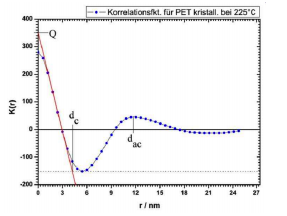
\includegraphics[width=0.4\textwidth]{img/autokorrel.png}
     \caption{Autokorrelationsfunktion für die Elektronendichte in PET am Beispiel einer bei 225°C kristallisierten Probe \cite{anleitung}.}
\end{figure}
\chapter{Durchführung}
\section{Präparation der PET-Probe}

Bei dem Material, welches in diesem Versuch untersucht wird, handelt es sich um Polyethylenterephtalat (PET), welches man in Form von Getränkeflaschen kennt und auch für die Herstellung von Folien und Fasern verwendet wird. Wir bedienen uns einer handelsüblichen PET-Flasche und schneiden kleine Stücke passend für den Probenhalter aus. Der Probenhalter ist ein längs geteiler Messingzylinder, in dessen Mitte ein längliches Messingplättchen einer Stärke von 1 mm mit rechteckiger Aussparung verschraubt wird. In dieser Aussparung fixieren und schmelzen/kristallisieren wir unsere Probe. Zur Fixierung dient Aluminiumfolie, die einmal um das Plättchen herumgelegt wird, nachdem das PET-Rohmaterial eingelegt worden ist. Nun legen wir das Plättchen auf eine Kochplatte und lassen es einige Zeit bei knapp unter 300 $^{\circ}$C schmelzen. Anschließend kommt die Probe für 10 Minuten (per Stoppuhr genau überprüft) bei 170 $^{\circ}$C in einen Ofen, um sie kristallisieren zu lassen. Nach Ablauf der 10 Minuten wird sie in kaltem Wasser abgeschreckt und ist nun nach Abtrocknung zur Messung bereit. 

Bei der Schmelze ist zu beachten, dass das PET verläuft und man deswegen die Menge nicht zu reichlich bemessen sollte, da es sonst aus der Aussparung überläuft, was in der Tat auch beinahe geschehen ist. Zudem hat sich gegen Ende der Schmelze eine bräunliche Verfärbung eingestellt, was zwei Gründe haben kann; zum einen hat der Schmelzvorgang deutlich länger angedauert als im Anleitungsblatt empfohlen, zum andern ist die Temperatur teilweise knapp über 300 $^{\circ}$C angestiegen. Zur Schmelzdauer ist zu sagen, dass die im Anleitungsblatt empfohlenen 5 Minuten etwas knapp bemessen sind, da die Wärmeleitung zwischen der Heizplatte und dem Probenhalter dazu nicht ausreicht, allerdings hat die tatsächliche Schmelze etwa 45 Minuten angedauert, was vermutlich wiederum zu lang ist (ideal sollten ca. 15-20 Minuten sein). Um die Temperatur konstant zu halten, ist es außerdem erforderlich, die Heizleistung der Platte nachzuregeln.

\section{Bestimmung der Positions des Primärstrahls}

Vor Beginn der eigentlichem Messung ist es notwendig, die Intensitätsverteilung des Primärstrahls zu bestimmen, da die Strichkollimation zwar gegenüber der Punktkollimation den Vorteil der generell höheren Intensität besitzt, jedoch das Strahlprofil nicht genau rechteckig ist, sondern abgerundet und zu den Rändern allmählich ausläuft. Aus diesem Grund müssen wir also zuerst eine Messung ohne Probe und ohne Primärstrahlfänger durchführen. Da ohne weitere Maßnahmen damit der empfindliche Szintillitationsdetektor zerstört werden würde, schalten wir den Messingabsorber vor die Strahlungsquelle dazu, der Strahl wird insgesamt also stark abgeschwächt. Zusätzlich montieren wir einen horizontalen Spalt mit einer Breite von 200 µm vor den Detektor. Das Innere der Kratky-Kamera wird anschließend evakuiert und eine winkelabhängige Messung der Intensität gestartet. 

Zuletzt setzen wir den Nullpunkt des Detektors auf das eben bestimmte Maximum des Primärstrahls, um die folgenden Messungen relativ dazu betrachten zu können.

\section{Hintergrundmessung mit leerem Probenhalter und Aluminiumfolie}

Um aus späteren Messungen die vom Probenbehlter und der Aluminiumfolie verursachte Hintergrundstrahlung herausrechnen zu können, war es notwendig, eine Messreihe mit einem leeren Probenbehälter durchzuführen. Dazu wurde der leere, mit Aluminiumfolie umwickelter, Probenbehälter in der Apparatur installiert, die Kratky-Kamera evakuiert und erneut eine winkelabhängige Messung der Intensität gestartet. Im Gegensatz zur Bestimmung des Primärstrahlprofils messen wir hier allerdings nur die gestreute Röntgenstrahlung, es wird also kein Absorber zur Abschwächung des Primärstrahls verwendet. Um dabei das Szintillatormessgerät nicht zu beschädigen, wird ein Primärstrahlfänger angebracht. Dieser ist so angebracht, dass der nicht abgelenkte Primärstrahl vollständig geblockt wird, die gestreute Strahlung allerdings ungehindert in den Szintillator eindringen kann.

\subsection{Wanderspaltmessung}

Zur Entschmierung der einzelnen Streudatenmessungen ist es notwendig, noch eine sogenannte Wanderspaltmessung durchzuführen. Dabei wird der zuvor angebrachte Horizontaler $200\mu m$ Spalt durch einen ebenfalls unbeweglichen $32 \mu m$ breiten vertikalen Spalt ausgetauscht. Zusätzlich wird vor der Probe ein beweglicher Spalt eingebracht. Dieser fährt in einem Zeitraum von 10 Sekunden von einer Seite des Primärstrahls zur anderen und anschließend mit gleicher Geschwindigkeit wieder zurück. Da bei dieser Messmethode nur ein sehr kleiner Teil der Strahlung beide Spalte passieren kann und statt der gestreuten Strahlung die Intensität des Primärstrahls gemessen wird, muss für die Wanderspaltmessung der Primärstrahlfänger entfernt werden.

Die Messung der Intensität erfolgt hierbei nicht winkelabhängig, statdessen wird pro Messung die Intensität des Primärstrahls über die gesamten 20 Sekunden aufgenommen den der bewegliche Spalt braucht, um wieder in die Startposition zurückzukehren.

Um den Fehler der Messung (Verursacht durch die statistische Natur der emittierten Röntgenstrahlung oder nicht gleichzeitigen Startens der Messung und des Spaltmotors) zu reduzieren, wird für jede Probe die Wanderspaltmessung 5 mal durchgeführt.

\clearpage{}
\section{Messungen mit Probe}

Analog zur winkelabhängigen- und Wanderspaltmessung mit der leeren Probe haben wir die Intensität des Primärstrahls mit der Wanderspalt-Messmethode sowie die winkelabhängige Intensität der gestreuten Strahlung für jede der uns zur Verfügung stehendenden Proben gemessen. Dabei ist anzumerken, dass bei der Messung der ersten Probe die Röntgenröhre ausgeschaltet war. Die Ursache für die Abschaltung ist uns nicht genau bekannt, eventuell ist jemand trotz aller Vorsicht versehentlich gegen den gelben Strom-Schalter für die Röntgenröhre gekommen.

Weiterhin wurde bei der Wanderspaltmessung wiederholt die Verbindung zwischen Messgerät und dem zur Auswertung benutzten Computer getrennt. Dies wurde vermutlich durch eine kleine Spannungsspitze beim Ein- oder Ausschalten des Motors für den beweglichen Spalt verursacht.

Die einzelnen Messungen wurde von uns in folgender Reihenfolge durchgeführt:


\begin{center}
  \begin{tabular}{|p{2.2cm}|p{4.5cm}|p{3cm}|p{4cm}|}
    \hline
    Messungs-Nummer & Kristallisationstemperatur der Probe in °C & Messmethode    & Name der Messdaten-Datei \\ \hline
    1               & 140                                        & Winkelabhängig & PET-140.0.txt \\ \hline
    2               & 140                                        & Wanderspalt    & PET-140.ms \\ \hline
    3               & 170                                        & Wanderspalt    & PET-170.ms \\ \hline
    4               & 170                                        & Winkelabhängig & PET-170.0.txt \\ \hline
    5               & 170 (Selbst getempert)                     & Winkelabhängig & PET-170-eigen.0.txt \\ \hline
    6               & 170 (Selbst getempert)                     & Wanderspalt    & PET-170-eigen.ms \\ \hline
    7               & 200                                        & Wanderspalt    & PET-200.ms \\ \hline
    8               & 200                                        & Winkelabhängig & PET-200.0.txt \\ \hline
    9               & 215                                        & Winkelabhängig & PET-215.0.txt \\ \hline
    10              & 215                                        & Wanderspalt    & PET-215.ms \\ \hline
	\end{tabular}
\end{center}

\chapter{Auswertung}
\section{Strahlcharakterisierung}

Folgende Grafik zeigt die Verteilung der Messereignisse in Abhängigkeit der vertikalen Detektorposition. Durch den horizontalen Spalt von 200 µm vor dem Detektor kann die Verteilung sehr genau über der Position aufgelöst werden. Wie zu sehen ist, liegt das Maximum bei 2050 µm und die Abnahme der Intensität ist nicht genau symmetrisch.

\begin{center}
\begin{figure}[h]
\begin{tikzpicture}
\begin{axis}[
    legend pos=south west,
    title={Messereignisse in Abhängigkeit der Detektorposition},
    xlabel=Detektorposition in µm,
    x tick label style={/pgf/number format/1000 sep=},
    ylabel=Messereignisse,
    y tick label style={/pgf/number format/1000 sep=},
    width=0.9\textwidth,
    height= 9cm,
    xmin=1500,
    xmax=2500,
    grid=both,
    ymin=0,
    %ymax=0.0045,
    tick align=outside,
    tickpos=left,
    minor x tick num=3,
    minor y tick num=4,
    minor grid style={dotted,thin}
]
\addplot[red, only marks, mark=x, mark size=1pt, %error bars/.cd, y dir=both, y fixed relative=0.01, x dir=both, x fixed=0.05
]
table[x index={0},y index={1}] {data/beamprofile2.bp};
%\addlegendentry{Leistung der LED auf der Photoplatte}
\end{axis}
\end{tikzpicture}
\captionof{figure}{Zahl der Messereignisse über der Detektorpositon mit leeren Probenhalter, ohne beamstop und mit Messing-Strahlabsorber.}
\end{figure}
\end{center}

\section{PET-Streudaten}
Mit Hilfe des Primärstralprofils und der Wanderspaltmessungen lassen sich die gemessenen Streudaten entschmieren, wodurch der Einfluss des nicht perfekt rechteckigen Strahlprofils herausrechnen lässt. Nach Entschmierung leifert das verwendete Messprogramm eine \.phg Datei, welche den Streuvektor q in inversen Angström, die Intensität in $e/nm^{3}$ und den Fehler der Inensität beinhaltet. Zur Darstellung und weiteren Verarbeitunt der Streudaten ist es vom Vorteil, den Streuvektor q in $s=\frac{q}{2\pi}$ umzurechnen und die Intensität mit $s^{2}$ multipliziert darzustellen.

\begin{figure}[h]
\begin{tikzpicture}
\begin{axis}[
  title={Streudaten für 140°C PET-Probe},
  Streudaten,
  name=first
]
\addplot[red, only marks, mark=x, mark size=2pt] table[x index=0,y index=1] {data/PET-140-nonFitPoints.rel};
\addlegendentry{Streudaten}
\addplot[green, only marks, mark=x, mark size=2pt] table[x index=0,y index=1] {data/PET-140-fitPoints.rel};
\addlegendentry{Untergrund}
\addplot[blue, mark=x, mark size=0pt, samples=20, domain=0:0.44] {225.817 * x^2};
\addlegendentry{Fitparabel}
\end{axis}

\begin{axis}[
  title={Streudaten für 170°C PET-Probe},
  Streudaten,
  name=second,
  at=(first.outer south east),
  anchor=outer south west
]
\addplot[red, only marks, mark=x, mark size=2pt] table[x index=0,y index=1] {data/PET-170-nonFitPoints.rel};
\addlegendentry{Streudaten}
\addplot[green, only marks, mark=x, mark size=2pt] table[x index=0,y index=1] {data/PET-170-fitPoints.rel};
\addlegendentry{Untergrund}
\addplot[blue, mark=x, mark size=0pt, samples=20, domain=0:0.44] {186.428 * x^2};
\addlegendentry{Fitparabel}
\end{axis}

\begin{axis}[
  title={Streudaten für 200°C PET-Probe},
  Streudaten,
  name=third,
  at=(first.outer south west),
  anchor=outer north west,
  yshift=-0.25cm
]
\addplot[red, only marks, mark=x, mark size=2pt] table[x index=0,y index=1] {data/PET-200-nonFitPoints.rel};
\addlegendentry{Streudaten}
\addplot[green, only marks, mark=x, mark size=2pt] table[x index=0,y index=1] {data/PET-200-fitPoints.rel};
\addlegendentry{Untergrund}
\addplot[blue, mark=x, mark size=0pt, samples=20, domain=0:0.44] {191.321 * x^2};
\addlegendentry{Fitparabel}
\end{axis}

\begin{axis}[
  title={Streudaten für 215°C PET-Probe},
  Streudaten,
  name=fourth,
  at=(third.outer south east),
  anchor=outer south west
]
\addplot[red, only marks, mark=x, mark size=2pt] table[x index=0,y index=1] {data/PET-215-nonFitPoints.rel};
\addlegendentry{Streudaten}
\addplot[green, only marks, mark=x, mark size=2pt] table[x index=0,y index=1] {data/PET-215-fitPoints.rel};
\addlegendentry{Untergrund}
\addplot[blue, mark=x, mark size=0pt, samples=20, domain=0:0.44] {208.726 * x^2};
\addlegendentry{Fitparabel}
\end{axis}

\end{tikzpicture}
\captionof{figure}{Streudaten der nicht von uns selbst hergestellten Proben. Zu erkennen ist ein von der Kristallisationstemperatur der Probe abhängender Peak und ein anschließender, annähernd parabelförmiger Anstieg der gemessenen Intensität.}
\end{figure}

\FloatBarrier

Wie an den Graphen zu erkennen ist, liegt in den gemessenen Daten eine gewisse Untergrundstrahlung vor, die parabelförmig zum Streuvektor zunimmt. Um die Messdaten weiter verarbeiten zu können, muss dieser Untergrund herausgerechnet werden. Dazu haben wir einen quadratischen fit durch die Messdaten und den Ursprung nach dem eigentlichen Peak gelegt (in den Graphen in grün gekennzeichnet) und von den gemessenen Daten abgezogen.

\subsection{Fitwerte}
Zur Bestimmung des Untergrunds haben wir eine Gerade der Form $f(x) = a \cdot x^2$ an die Streudaten hinter dem Peak angefittet. Die für den Fit verwendete Messdaten sind in den oben dargestellten Graphen grün markiert.

\begin{center}
  \begin{tabular}{|p{7cm}|p{2.2cm}|p{2.2cm}|}
    \hline
    Kristallisierungstemperatur der Probe & a     & Fehler $\Delta$a  \\ \hline
    140                                   & 225,8 & 25,6              \\ \hline
    170                                   & 186,4 & 31,3              \\ \hline
    170 (selbst getempert)                & 132,4 & 33,4              \\ \hline
    200                                   & 191,3 & 32,9               \\ \hline
    215                                   & 208,7 & 25,7              \\ \hline
	\end{tabular}
\end{center}

Aufgrund der sehr hohen Streuung der hinteren Messwerte sind die resultierenden Fits wie erwartet mit einem relativ großen Fehler behaftet.


\section{Eindimensionale Korrelationsfunkton}
Die um den linearen Anteil korrigierten Streudaten können nun mit Hilfe des Programms "`CORREL1"' mittels Furiertransformation in eine Autokorrelationsfunktion umgerechnet werden. Mit Hilfe dieser Funktion ist es möglich, werte Für $Q$, $d_c$ und $d_{ac}$ für die einzelnen Probem zu bestimmen.

Dazu wird durch den anfänglich linear abfallenden Teil eine Fitgerade gelegt. Der y-Achsenabschnitt dieser Gerade gibt uns den Wert für Q, welcher sich in den gesuchten Wert $\Phi_c$ für die Kristallinität der Probe umrechnen lässt. Den Wert für $d_c$ ist der x-Wert des Schnittpunktes der fitgeraden mit einer Konstanten, die durch den tiefsten Punkt der Autokorrelationsfunktion verläuft. Den Wert für $d_{ac}$ erhält man aus dem x-Wert des ersten lokalen Maximums der Elektronendichte-Autokorrelationsfunktion.

\begin{figure}[h]
\begin{tikzpicture}
\begin{axis}[
  title={Autokor.\ für PET Kristall bei 140°C},
  Autokorrel,
  name=first
]
\addplot[red, only marks, mark=x, mark size=2pt] table[x index=0,y index=1] {data/PET-140.cor};
\addlegendentry{Autokorrelationsfunktion}

\addplot[black, mark=x, mark size=0pt, samples=20, domain=0:25] {0};

\addplot[blue, mark=x, mark size=0pt, samples=20] {170.514 - 73.9278*x};
\addplot[blue, mark=x, mark size=0pt, samples=20, domain=0:25] {-71.1939};
\draw (axis cs:3.2695187238902865, -71.1939) -- (axis cs:3.2695187238902865,0) node [above] {$d_c$};
\draw (axis cs:9.62545,0) -- (axis cs:9.62545,17.4268) node [above] {$d_{ac}$};
\addlegendentry{Fitgerade}
\end{axis}


\begin{axis}[
  title={Autokor.\ für PET Kristall bei 170°C},
  Autokorrel,
  name=second,
  at=(first.outer south east),
  anchor=outer south west
]
\addplot[red, only marks, mark=x, mark size=2pt] table[x index=0,y index=1] {data/PET-170.cor};
\addlegendentry{Autokorrelationsfunktion}

\addplot[black, mark=x, mark size=0pt, samples=20, domain=0:25] {0};
\addplot[blue, mark=x, mark size=0pt, samples=20] {208.317 - 80.5536*x};
\addplot[blue, mark=x, mark size=0pt, samples=20, domain=0:25] {-95.4946};
\draw (axis cs:3.771545796842133,-95.4946) -- (axis cs:3.771545796842133,0) node [above] {$d_c$};
\draw (axis cs:10.8286,0) -- (axis cs:10.8286,22.8436) node [above] {$d_{ac}$};
\addlegendentry{Fitgerade}
\end{axis}

\begin{axis}[
  title={Autokor/. für eigenen PET Kristall bei 170°C},
  Autokorrel,
  name=third,
  at=(first.outer south west),
  anchor=outer north west,
  yshift=-0.25cm
]
\addplot[red, only marks, mark=x, mark size=2pt] table[x index=0,y index=1] {data/PET-170-eigen.cor};
\addlegendentry{Autokorrelationsfunktion}

\addplot[black, mark=x, mark size=0pt, samples=20, domain=0:25] {0};
\addplot[blue, mark=x, mark size=0pt, samples=20] {193.859 - 63.7651*x};
\addplot[blue, mark=x, mark size=0pt, samples=20, domain=0:25] {-84.106};
\draw (axis cs:4.3591951581626125,-84.106) -- (axis cs:4.3591951581626125,0) node [above] {$d_c$};
\draw (axis cs:12.6334,0) -- (axis cs:12.6334,19.592) node [above] {$d_{ac}$};
\addlegendentry{Fitgerade}
\end{axis}

\begin{axis}[
  title={Autokor.\ für PET Kristall bei 200°C},
  Autokorrel,
  name=fourth,
  at=(third.outer south east),
  anchor=outer south west
]
\addplot[red, only marks, mark=x, mark size=2pt] table[x index=0,y index=1] {data/PET-200.cor};
\addlegendentry{Autokorrelationsfunktion}

\addplot[black, mark=x, mark size=0pt, samples=20, domain=0:25] {0};
\addplot[blue, mark=x, mark size=0pt, samples=20] {210.18 - 69.4293*x};
\addplot[blue, mark=x, mark size=0pt, samples=20, domain=0:25] {-87.1074};
\draw (axis cs:4.281867365438092,-87.1074) -- (axis cs:4.281867365438092,0) node [above] {$d_c$};
\draw (axis cs:13.235,0) -- (axis cs:13.235,18.3741) node [above] {$d_{ac}$};
\addlegendentry{Fitgerade}
\end{axis}

\begin{axis}[
  title={Autokor.\ für PET Kristall bei 215°C},
  Autokorrel,
  name=fith,
  at=(third.outer south west),
  anchor=outer north west,
  yshift=-0.25cm
]
\addplot[red, only marks, mark=x, mark size=2pt] table[x index=0,y index=1] {data/PET-215.cor};
\addlegendentry{Autokorrelationsfunktion}

\addplot[black, mark=x, mark size=0pt, samples=20, domain=0:25] {0};
\addplot[blue, mark=x, mark size=0pt, samples=20, domain=0:6] {132.197 - 36.1102*x};
\addplot[blue, mark=x, mark size=0pt, samples=20, domain=0:25] {-44.4861};
\draw (axis cs:4.892873947051315,-44.4861) -- (axis cs:4.892873947051315,0) node [above] {$d_c$};
\draw (axis cs:15.0398,0) -- (axis cs:15.0398,6.98367) node [above] {$d_{ac}$};
\addlegendentry{Fitgerade}
\end{axis}

\begin{axis}[
  title={Autokorrelationsfunktionen},
  Autokorrel,
  name=sixth,
  at=(fith.outer south east),
  anchor=outer south west
]
\addplot[red, smooth, mark=x, mark size=0pt] table[x index=0,y index=1] {data/PET-140.cor};
\addlegendentry{140°C}
\addplot[green, smooth, mark=x, mark size=0pt] table[x index=0,y index=1] {data/PET-170.cor};
\addlegendentry{170°C}
\addplot[blue, smooth, mark=x, mark size=0pt] table[x index=0,y index=1] {data/PET-170-eigen.cor};
\addlegendentry{170°C (eigen)}
\addplot[purple, smooth, mark=x, mark size=0pt] table[x index=0,y index=1] {data/PET-200.cor};
\addlegendentry{200°C}
\addplot[orange, smooth, mark=x, mark size=0pt] table[x index=0,y index=1] {data/PET-215.cor};
\addlegendentry{215°C}
\addplot[black, mark=x, mark size=0pt, samples=20, domain=0:25] {0};
\end{axis}

\end{tikzpicture}
\captionof{figure}{Autokorrelationsfunktionen der untersuchten Proben. Mit hilfe eines linearen fits im vorderen Bereich der Funktion lassen sich Werte für Q und $d_c$ bestimmen. Der Wert für $d_{ac}$ ergibt sich aus der Position des ersten lokalen Maximums}
\end{figure}
\FloatBarrier
Aus den Autokorrelationsfunktionen lassen sich folgende Werte für die uns zur verfügung stehenden Proben entnehmen:

\begin{center}
  \begin{tabular}{|p{4.5cm}|p{2.6cm}|p{2.6cm}|p{2.6cm}|p{2.6cm}|}
    \hline
    Kristallisierungstemperatur der Probe in °C & $d_c$ in $nm$   & $d_{ac}$ in $nm$ & $Q$         & $ \Phi_c in \%$ \\ \hline
    140                                         & $3,27 \pm 0,04$ & $ 9,6 \pm 0,5$   & $171 \pm 5$ & $14,1 \pm 0,5$  \\ \hline
    170                                         & $3,77 \pm 0,06$ & $10,8 \pm 0,5$   & $208 \pm 8$ & $18,0 \pm 0,9$  \\ \hline
    170 (selbst getempert)                      & $4,36 \pm 0,06$ & $12,6 \pm 0,6$   & $194 \pm 6$ & $16,4 \pm 0,7$  \\ \hline
    200                                         & $4,28 \pm 0,07$ & $13,2 \pm 0,7$   & $210 \pm 8$ & $18,2 \pm 1,0$  \\ \hline
    215                                         & $4,89 \pm 0,06$ & $15,0 \pm 0,8$   & $132 \pm 4$ & $10,5 \pm 0,3$  \\ \hline
	\end{tabular}
\end{center}

Man kann nun sowohl die Kristallitdicke als auch die Langperiode gegenüber der Differenz zwischen der Kristallisationstemperatur der Proben und dem Schmelzpunkt des Materials auftragen. Zu erwarten ist hier eine $\frac{1}{T}$ Abhängigkeit für die Kristallitdicke und eine $\frac{1}{\sqrt{T}}$ Abhängigkeit für die Langperiode.
\FloatBarrier


\begin{figure}[h]
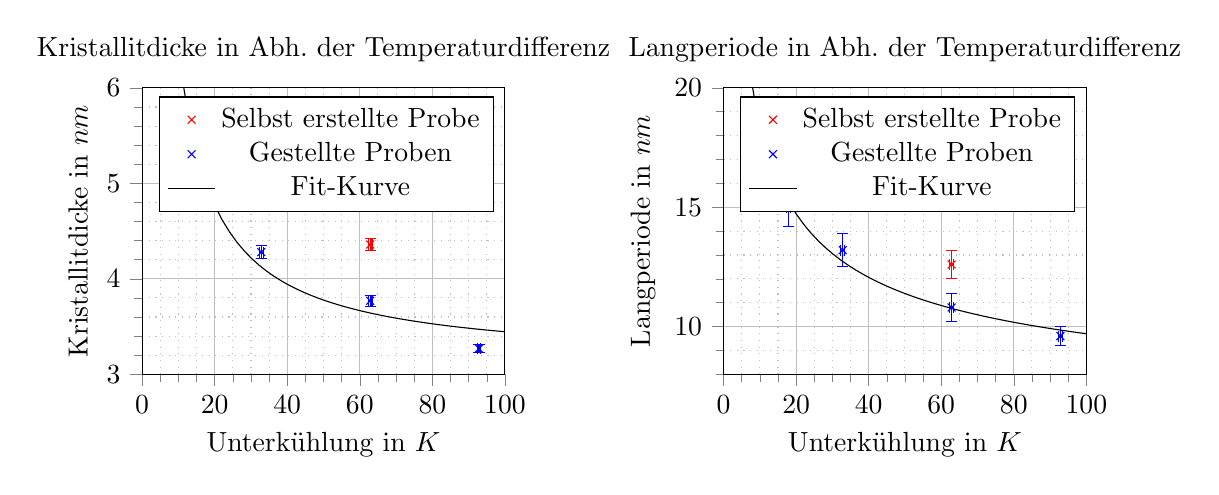
\begin{tikzpicture}
\begin{axis}[
  title={Kristallitdicke in Abh.\ der Temperaturdifferenz},
  ylabel=Kristallitdicke in $nm$,
  tabh,
  name=first
]
\addplot[red, only marks, mark=x, mark size=2pt, 
  error bars/.cd, y dir=both,y explicit, x dir=both,x explicit]
  coordinates{%
    (62.85,4.36) +- (0.5, 0.06)
  };
\addlegendentry{Selbst erstellte Probe}
\addplot[blue, only marks, mark=x, mark size=2pt, 
  error bars/.cd, y dir=both,y explicit, x dir=both,x explicit]
  coordinates{%
    (17.85,4.89) +- (0.5, 0.06)
    (32.85,4.28) +- (0.5, 0.07)
    (62.85,3.77) +- (0.5, 0.06)
    (92.85,3.27) +- (0.5, 0.04)
  };
\addlegendentry{Gestellte Proben}

\addplot[black, mark=x, mark size=0pt, samples=20, domain=0:20] {3.1144 + 33.1644/x};
\addplot[black, mark=x, mark size=0pt, samples=40, domain=20:100] {3.1144 + 33.1644/x};
\addlegendentry{Fit-Kurve}
\end{axis}


\begin{axis}[
  title={Langperiode in Abh.\ der Temperaturdifferenz},
  tabh,
  ylabel=Langperiode in $nm$,
  ymin=8,
  ymax=20,
  name=second,
  at=(first.outer south east),
  anchor=outer south west
]
\addplot[red, only marks, mark=x, mark size=2pt, 
  error bars/.cd, y dir=both,y explicit, x dir=both,x explicit]
  coordinates{%
    (62.85,12.6) +- (0.5, 0.6)
  };
\addlegendentry{Selbst erstellte Probe}
\addplot[blue, only marks, mark=x, mark size=2pt, 
  error bars/.cd, y dir=both,y explicit, x dir=both,x explicit]
  coordinates{%
    (92.85, 9.6) +- (0.5, 0.4)
    (62.85,10.8) +- (0.5, 0.6)
    (32.85,13.2) +- (0.5, 0.7)
    (17.85,15) +- (0.5, 0.8)
  };
\addlegendentry{Gestellte Proben}

\addplot[black, mark=x, mark size=0pt, samples=20, domain=0:20] {5.63251 + 40.6655/x^0.5};
\addplot[black, mark=x, mark size=0pt, samples=40, domain=20:100] {5.63251 + 40.6655/x^0.5};
\addlegendentry{Fit-Kurve}
\end{axis}
\end{tikzpicture}
\captionof{figure}{}
\end{figure}
\FloatBarrier
Es ist auffällig, dass die von uns hergestellte, in rot markierte Probe in keinem der Graphen zu den erwarteten Werten passt. Dies kann in der bereits in der Durchführung erwähnten zu hohen Temperatur, die zum Schmelzen des PET-Materials verwendet wurde, begründet sein.

Für die uns gestellten Proben passt die erwartete $\frac{1}{\sqrt{T}}$ Abhängigkeit der Langperiode zur Kristallisationstemperatur hier sehr gut zu den aufgenommenen Messdate, während die gemessenen Punkte für die Kristallitdicke größtenteils abseits der $\frac{1}{T}$ Kurve liegen.

\clearpage{}

Zur Auswertung des Kristallationsgrades der Proben in Abhängigkeit zur Kristallisationstemperatur haben wir einen Fit der Form $\Phi(T) = a \cdot e^{-\frac{B_0}{T^{\infty}_{f}-T}-\frac{T_A}{T-T_V}}$ \cite{anleitung} durch die uns zur Verfügung stehenden Messdaten gelegt. Für $T^{\infty}_{f}$ haben wir den Schmelzpunkt von $T_s = 506K$ des Materials und für $T_V$ haben wir $T_G - 50K = 293K$ angenommen. Für die Aktivierungstemperatur $T_A$ haben wir zuerst gemäß der Versuchsanleitung Werte zwischen $1000K$ und $2000K$ verwendet, da uns ein Literaturwert nicht zur Verfügung stand. Das erste Diagramm zeigt einen Fit für $T_A = 1500K$, welcher jedoch nicht die gemessenen Werte widerspiegelt. Aus diesem Grund haben wir einen weiteren Fit mit $T_A$ als zusätzlichen Fitparameter erstellt.

\begin{figure}[h]
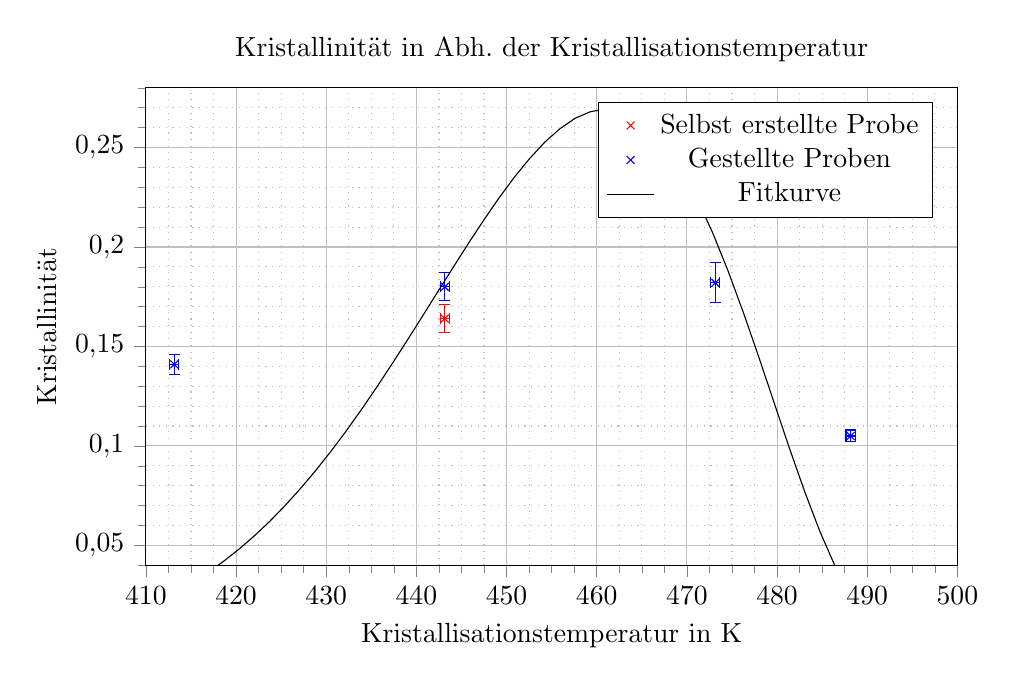
\begin{tikzpicture}
\begin{axis}[
  title={Kristallinität in Abh.\ der Kristallisationstemperatur},
  /pgf/number format/use comma,
  ylabel=Kristallinität,
  legend pos=north east,
  x tick label style={/pgf/number format/1000 sep=},
  xlabel=Kristallisationstemperatur in K,
  y tick label style={/pgf/number format/1000 sep=},
  yticklabel style={/pgf/number format/fixed},
  width=0.85\linewidth,
  height=0.5\linewidth,
  scale only axis,
  xmin=410,
  xmax=500,
  grid=both,
  ymin=0.04,
  ymax=0.28,
  tick align=outside,
  tickpos=left,
  minor x tick num=3,
  minor y tick num=4,
  minor grid style={dotted,thin}
]
\addplot[red, only marks, mark=x, mark size=2pt, 
  error bars/.cd, y dir=both,y explicit, x dir=both,x explicit]
    coordinates{%
    (170+273.15,0.164)   +- (0.5, 0.007)
  };
\addlegendentry{Selbst erstellte Probe}
\addplot[blue, only marks, mark=x, mark size=2pt, 
  error bars/.cd, y dir=both,y explicit, x dir=both,x explicit]
  coordinates{%
    (140+273.15,0.141) +- (0.5, 0.005)
    (170+273.15,0.180) +- (0.5, 0.007)
    (200+273.15,0.182) +- (0.5, 0.010)
    (215+273.15,0.105) +- (0.5, 0.003)
  };
\addlegendentry{Gestellte Proben}

\addplot[black, mark=x, mark size=0pt, samples=60, domain=400:500] {21924.3 * e^(-(107.068/(506-x))-1500/(-293+x))};
\addlegendentry{Fitkurve}
\end{axis}
\end{tikzpicture}
\captionof{figure}{Starke Diskrepanz zwischen Fitkurve und gemessenen Daten bei angenommener Aktivierungstemperatur von $T_A = 1500K$, ein ähnlicher Verlauf findet sich für andere Werte von $T_A$ zwischen $1000K$ und $2000K$}
\end{figure}

\begin{figure}[h]
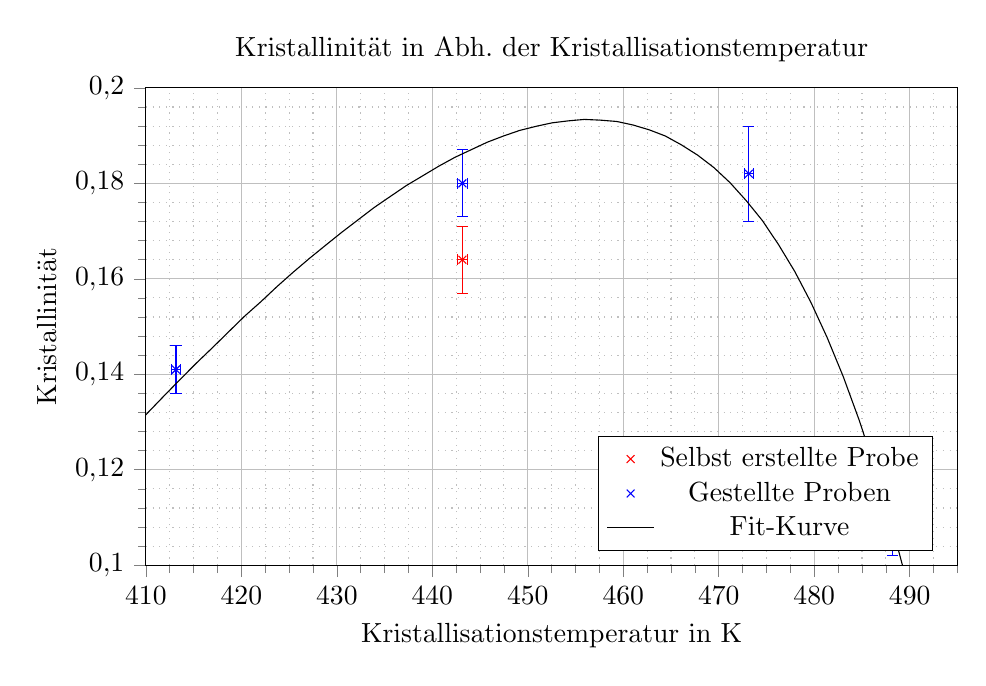
\begin{tikzpicture}
\begin{axis}[
  title={Kristallinität in Abh.\ der Kristallisationstemperatur},
  /pgf/number format/use comma,
  ylabel=Kristallinität,
  legend pos=south east,
  x tick label style={/pgf/number format/1000 sep=},
  xlabel=Kristallisationstemperatur in K,
  y tick label style={/pgf/number format/1000 sep=},
  yticklabel style={/pgf/number format/fixed},
  width=0.85\linewidth,
  height=0.5\linewidth,
  scale only axis,
  xmin=410,
  xmax=495,
  grid=both,
  ymin=0.10,
  ymax=0.20,
  tick align=outside,
  tickpos=left,
  minor x tick num=3,
  minor y tick num=4,
  minor grid style={dotted,thin}
]
\addplot[red, only marks, mark=x, mark size=2pt, 
  error bars/.cd, y dir=both,y explicit, x dir=both,x explicit]
    coordinates{%
    (170+273.15,0.164)   +- (0.5, 0.007)
  };
\addlegendentry{Selbst erstellte Probe}
\addplot[blue, only marks, mark=x, mark size=2pt, 
  error bars/.cd, y dir=both,y explicit, x dir=both,x explicit]
  coordinates{%
    (140+273.15,0.141) +- (0.5, 0.005)
    (170+273.15,0.180) +- (0.5, 0.007)
    (200+273.15,0.182) +- (0.5, 0.010)
    (215+273.15,0.105) +- (0.5, 0.003)
  };
\addlegendentry{Gestellte Proben}

\addplot[black, mark=x, mark size=0pt, samples=60, domain=400:500] {1.44075 * e^(-(23.1857/(506-x))-251.81/(-293+x))};
\addlegendentry{Fit-Kurve}
\end{axis}
\end{tikzpicture}
\captionof{figure}{Wird $T_A$ als Fitparameter gewählt, ergibt sich mit $T_A = (251,81 \pm 51,1454)K$ eine deutliche Abdeckung mit den gemessenen Daten.}
\end{figure}
\FloatBarrier

Auch hier passt der Datenpunkt der von uns hergestellten Probe nicht zum erwarteten Wert, wobei es sinnig erscheint, dass bei einem "`Verbrennen"' der Probe die Kristallinität gegenüber einer sauber geschmolzenen Probe abnimmt. Beispielsweise ist vorstellbar, dass die Molekülketten im Polymer aufgrund der erhöhten Temperatur vermehrt auseinanderfallen, demzufolge kürzere Ketten vorliegen, wodurch dann die Anzahl der amorphen Randbereiche gegenüber der Zahl der geordneten, parallel liegenden Ketten zunimmt. Es ist natürlich auch möglich dass das Tempern im Ofen zu kurz angedauert hat und somit die Probe zu wenig Zeit zum Kristallisieren hatte.

\clearpage{}
\subsection{Fitwerte}

Für den Fit der Kristallitdicke haben wir eine Funktion der Form $f\left(x\right) = \frac{a}{T} + b$ zu Grunde gelegt. Es ergeben sich folgende Fitwerte:
\begin{center}
  \begin{tabular}{|p{1.5cm}|p{1.5cm}|p{1.5cm}|}
    \hline
    Parameter & Wert    & Fehler \\ \hline
    a         & 33,2   & 6,0   \\ \hline
    b         & 3,1    & 0,2   \\ \hline
	\end{tabular}
\end{center}

Für die Langperiode wurde eine Funktion der Form $f\left(x\right)  = \frac{a}{\sqrt{T}} + b$ zu Grunde gelegt. Folgende Werte haben wir bestimmt:
\begin{center}
  \begin{tabular}{|p{1.5cm}|p{1.5cm}|p{1.5cm}|}
    \hline
    Parameter & Wert    & Fehler \\ \hline
    a         & 40,7   & 4,1   \\ \hline
    b         & 5,6    & 0,7   \\ \hline
	\end{tabular}
\end{center}

Zum fitten der Kristallinität in Abhängigkeit der Temperatur wurde zuerst $\Phi(T) = a \cdot e^{-\frac{B_0}{506K-T}-\frac{1500K}{T-293K}}$ als Funktion verwendet. Dies liefert folgende Fit-Parameter:

\begin{center}
  \begin{tabular}{|p{1.5cm}|p{1.5cm}|p{1.5cm}|}
    \hline
    Parameter & Wert  & Fehler \\ \hline
    $a$       & 21924 & 36395  \\ \hline
    $B_0$     & 107   & 66     \\ \hline
	\end{tabular}
\end{center}

Weiterhin haben wir die Aktivierungstemperatur $T_A$ als weiteren Fitparameter gewählt: $\Phi(T) = a \cdot e^{-\frac{B_0}{506K-T}-\frac{T_A}{T-293K}}$ als Funktion verwendet. Dies liefert folgende Fit-Parameter:

\begin{center}
  \begin{tabular}{|p{1.5cm}|p{1.5cm}|p{1.5cm}|}
    \hline
    Parameter & Wert  & Fehler \\ \hline
    $a  $     & 1,44  & 0,60   \\ \hline
    $B_0$     & 23.2  & 4,0    \\ \hline
    $T_A$     & 251,8 & 51,2   \\ \hline
	\end{tabular}
\end{center}

\chapter{Fazit}

Wir haben in diesem Versuch den Kristallisationsgrad von verschiedenen Polymerproben in Abhängigkeit der Temperaturen, bei denen das Material kristallisiert ist, untersucht. Dazu wurden aus den Streuwinkelmessungen die zugehörigen Autokorrelationsfunktionen (nach Bereinigung der Werte) ermittelt und daraus die charakteristischen Größen berechnet bzw.\ abgeschätzt, die es uns letztlich ermöglicht haben die Kristallinität zu berechnen. Die selbst hergestellte Probe scheint zwar aufgrund der Messwerte nicht ideal gelungen zu sein, jedoch war die Ermittlung der Kristallinität weitestgehend erfolgreich und es stellt sich auch klar eine Temperaturabhängigkeit der Kristallinität heraus. Es zeigt sich, dass die Messmethode mittels Röntgenkleinwinkelstreuung grundsätzlich geeignet ist, das Kristallisationsverhalten der Polymerproben zu ermitteln, allerdings weicht die Auswertung der Messdaten von der Theorie ab, die zur Vorbereitung der Kristallinitätsberechnung herangezogen wurde (vgl.\ obige Abweichung der Fitparameter). 

%ENDE INHALT
\cleardoublepage{}
% Eintrag fürs Inhaltsverzeichnis
\newpage
\begin{thebibliography}{100}
  \bibitem{anleitung} \url{Versuchsanleitung}
\end{thebibliography}
\end{document}
